\documentclass[11pt,letter]{article}

\usepackage{amsmath}
\usepackage{amssymb}
\usepackage{graphicx}
\usepackage{caption}
\usepackage{subfig}
\usepackage{setspace}
\onehalfspacing
\usepackage{fullpage}

\begin{document}

\title{CS182 Final Project Report:\\
100,000 Asteroids Down the Back of The Couch}
\author{Paul Blankley, Matthew Holman, Ryan Janssen}
\date{Due: December 8, 2017}
\maketitle 

\section*{Background: The Minor Planet Center}
The Minor Planet Center (MPC), at the Harvard-Smithsonian Center for Astrophysics, is the world's clearinghouse for asteroid observations.  The MPC collects in real-time data from hundreds to thousands of observing sites, roughly $10^5$ individual observations per night.  The data are archived, processed, and served back to the public and researchers with a primary goal: facilitating the rapid detection and characterization of near-Earth objects (NEOs).  The MPC is one of a number of NASA-funded facilities working toward fulfilling a US Congressional mandate of finding 90\% of potentially hazardous NEOs that have estimated diameters greater than 140m.

The MPC archives currently contain over 170 million individual observations of $\sim700K$ distinct objects.  Observations reported to the MPC pass through a number of processing steps:

\begin{itemize}
    \item Validation and archiving.  Improperly formatted or physically implausible observations are returned.  Valid observations are archived in their original form.
    \item Identification.  Observations are checked to see if they match the predicted locations of known objects with well-determined orbits.  Identified observations are set aside for later processing.
    \item Classification.  Tracklets that display rapid motion are often near-Earth objects.  These are prioritized for additional observations because they can be lost if not observed immediately.
    \item Linking.  Separate tracklets of the same object are matched together.  We do not know {\it a priori} which tracklets go together.  Plausible matches are hypothesized and then tested with orbit fitting.
\end{itemize}

\section*{The Problem: The Isolated Tracklet File (ITF)}
\subsection*{What is the ITF?}
The observations reported to the MPC follow a fixed 80-character format that originated in the era of punch cards.  As an example, here are the first few observations of A/2017 U1, the recently discovered interstellar object:

\begin{verbatim}
    AK17U010  C2017 10 18.47298 01 59 57.442+02 06 04.30         19.8 wLEU183F51
    AK17U010  C2017 10 18.49990 01 59 08.910+02 07 20.19               LEU183F51
    AK17U010  C2017 10 19.39715 01 34 55.362+02 45 03.20         19.9 wLEU183F51
    AK17U010  C2017 10 19.40837 01 34 38.745+02 45 28.24         19.9 wLEU183F51
    AK17U010  C2017 10 19.41968 01 34 21.948+02 45 53.55         20.1 wLEU183F51
\end{verbatim}

The first few characters are the unique designation of the object (in compact form).  The `C' indicates CCD digital observations.  Next are the year, month, and fractional day.  Following that are the right ascension and declination (longitude and latitude on sky), the magnitude (a measure of brightness), filter, and observatory code (the `F51' at the end means the Pan-STARRS-1 observatory on Hale'akala, Maui.  This information specifies what object was observed, its observed location and brightness at each time, and where it was observed from.  

These observations are grouped by the observers into `tracklets' (Kubica et al. 2017).  A tracklet is a collection of two or more observations taken over a short enough time span (minutes to hours) that the observer is confident that the observations are real rather than spurious and that they represent the same object.  Tracklets normally exhibit linear, constant-rate motion within the span of a few hours.

Roughly 90\% of the observations reported to the MPC can be immediately identified as known objects.  And of the remaining 10\%, most can be linked with other tracklets reported within the past few days.  However, some tracklets cannot be identified or linked.  These end up in the {\it Isolated Tracklet File} or ITF.

The ITF currently contains about fourteen million observations grouped into about three million tracklets.  Most of those tracklets are real.  And given the area of sky observed nightly by large NASA-funded surveys, we can estimate that most objects have been observed multiple times.  It is not uncommon for nearly discovered objects, with well-determined orbits, to match several tracklets in the ITF, spread out of the course of years.  

\subsection*{A challenging problem}
As telescope apertures increase, the number of tracklets stored in the ITF continues to grow.  To satisfy the Congressional mandate, we will ultimately require a methodology to link ITF tracklets into full asteroid orbits.

This is a not a toy problem - the ITF is in fact a real data set that is as of yet unsolved.  The challenges with processing the ITF are numerous:

\begin{itemize}
    \item \textbf{Large state space:}
    The brute force solution is to pair every tracklet in the ITF with every other tracklet, and run an orbit-fitting algorithm to test the match.  Then, check the plausible matches with other tracklets to see if a third, fourth, fifth, etc., tracklet also matches (multiple matches are required for sufficient confidence levels).  As we would need to iterate this process over 3 million tracklets, the brute force method is computationally difficult.
    \item \textbf{Partial data:}
    Each asteroid has six orbital parameters (three position components and three velocity components).  Observations of a single tracklet provide four of these (a starting location and two rates of motion on the sky plane), but the radial distance and velocity from the observer are not directly observed.   Thus, asteroids cannot be matched simply by comparing parameters.  The fundamental challenge in the linking problem, and orbit fitting in general, is inferring the distance to the observed object at the time of the observations. 
    \item \textbf{High asteroid density:}
    In any given region of the night sky, many asteroids can be observed (several tens per square degree for the brightness limits of current surveys).  As a result, clustering algorithms must be carefully designed and tuned to avoid false positive clusters.
    \begin{figure}[!hp]%
    \centering
    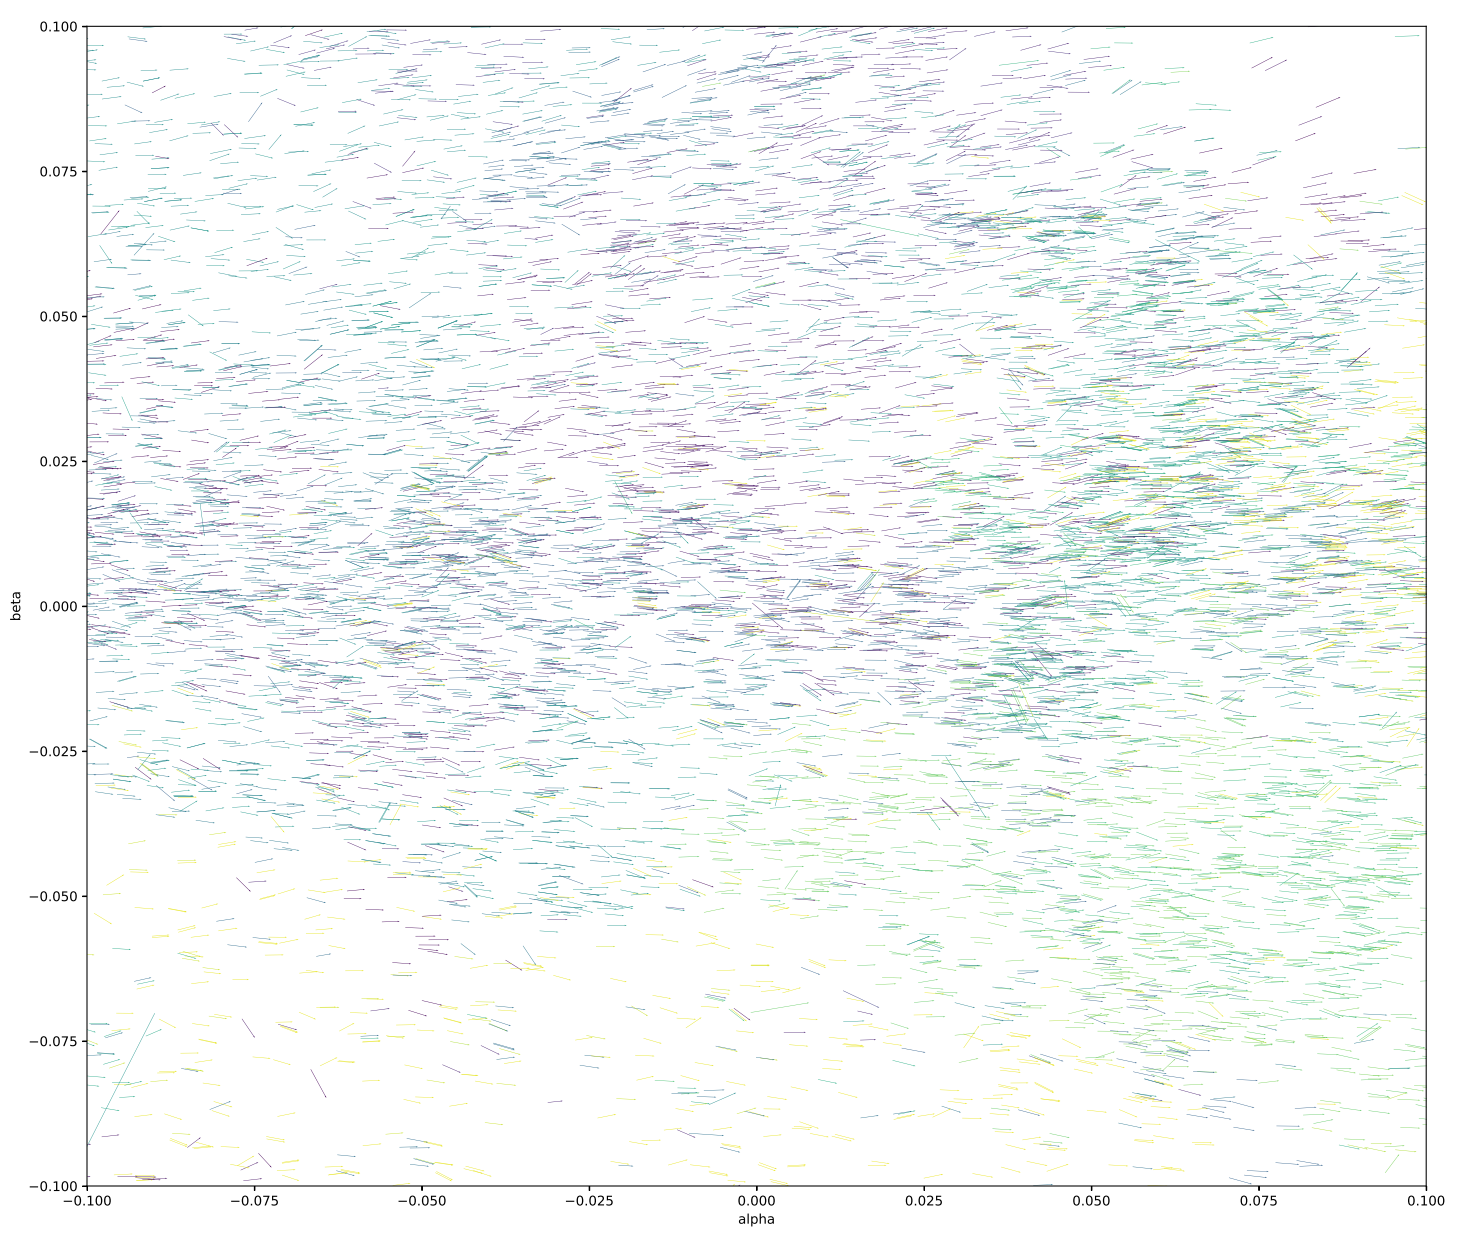
\includegraphics[width=10cm]{3_Final_write_up/6_ITG_img.png}
    \caption{Sample ITF tracklet density - 30 days of observations in a small portion of the night sky}%
    \label{fig:itf_sample}%
\end{figure}
    \item \textbf{Large time separation:}
    In the ITF, observations are sparse in time; this makes it difficult to 'connect the dots' by just looking which tracklets are nearby.
    \item \textbf{Highly nonlinear:}
    When observed from the moving reference from of the earth, asteroids follow a highly non-linear trajectory across the sky.  This necessitates complex curve-fitting algorithms, compounding the issues of computational tractability.
\end{itemize}

We originally proposed to apply the graph search algorithms we  learned in class to this problem.  The goal was, and still is, to link as many tracklets in the ITF as possible, using as few expensive orbit-fitting calculations as possible.  Our objective for the project was to identify at least 5 new objects from the ITF.  However, if we can structure an efficient and complete heuristic, our aspirational result could be a nearly-complete partitioning of the ITF into disjoint sets of tracklets that represent the same physical object, along with measures of confidence that the tracklets in each set indeed go together.

\section*{Current Solutions for Isolated Tracklets}
There have been previous attempts to maps unlinked asteroid tracklets, notably PanSTARRS
(Kaiser et al. 2002; Hodapp et al. 2004), and the Moving Object Processing System (MOPS, Denneau et al. 2013).  In particular, MOPS had some success with identifying clusters, also using a KD-tree clustering methodology.  However, they have had challenges on two fronts:
\begin{itemize}
    \item \textbf{Computational efficiency:}
    MOPS's approach requires computationally expensive orbit-fitting calculations for each of candidate link. We believe that with the MOPS methodology the number of candidate links scales as $O(n^3)$, making it computationally difficult for the present number of asteroid tracklets.
    \item \textbf{False Positives:}
    Veres and Chesley (submitted to AJ, 2017) note that MOPS performed better for low density state spaces, and that for higher object densities spurious detections were a significant problem.
\end{itemize}    
Each of these two challenges will grow as improved asteroid detection continues to increase both the number and density of tracklets.  To date, we know of no successes identifying missing asteroids from the ITF on a large scale.
    

\section*{Our Approach: Heliocentric-based clustering}
Our core intuition to speeding up the problem is to use something called `heliocentric linking.'\newline 
The idea is to posit a radial distance/velocity to the observed objects,  transform the data as if observing from the sun, and then look for tracklets that occupy the same great circle on the sky.
Asserting the heliocentric radial distance gives us both a complete position and velocity vector for each tracklet, which we can project to a common time.  Asteroids that have the same orbit should have the same position and velocity at a reference time.  This allows us to cluster tracklets, given the assumed distance.
\begin{figure}[!hp]%
    \centering
    \subfloat[Section of sky at inferred $\dot{z} = \dot{z_1}$]{{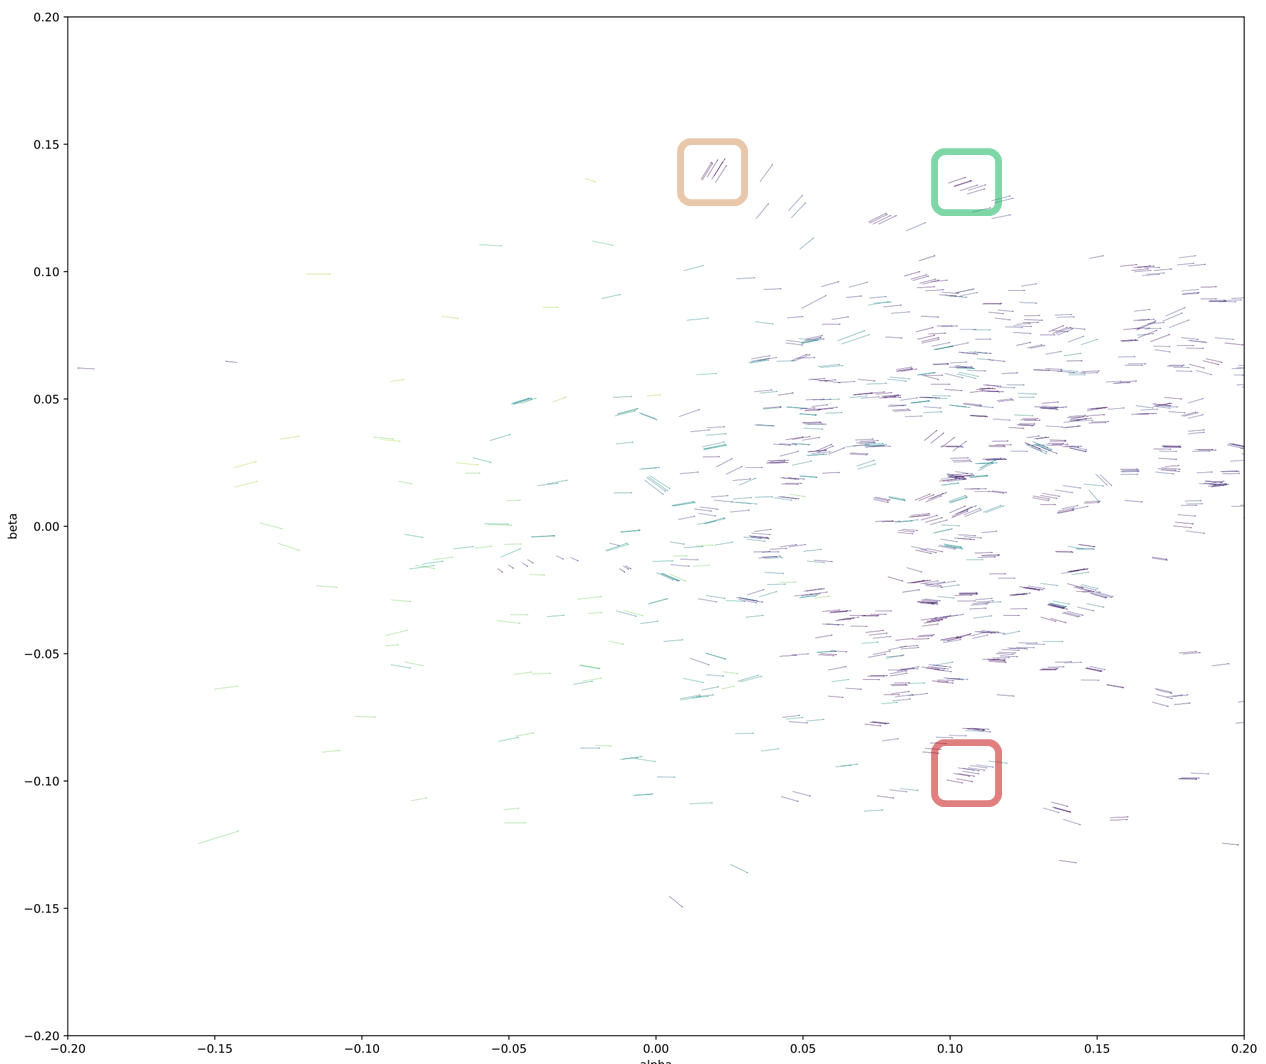
\includegraphics[width=7cm]{3_Final_write_up/2a_lens1_img.png} }}%
    \qquad
    \subfloat[Same section of sky at inferred $\dot{z} = \dot{z_2}$]{{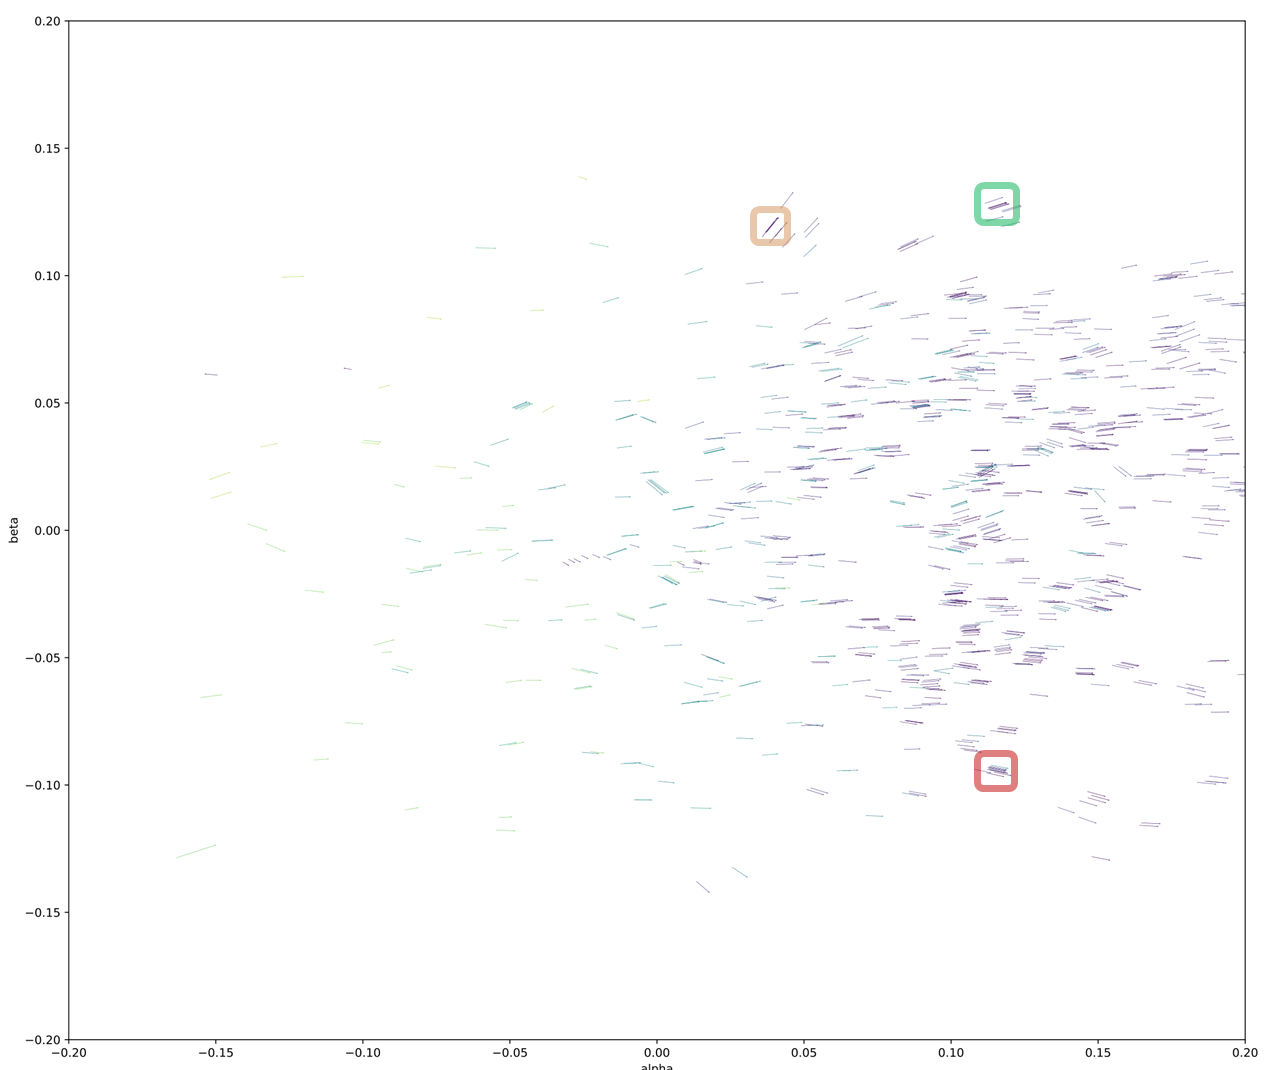
\includegraphics[width=7cm]{3_Final_write_up/2b_lens2_img.png} }}%
    \caption{Several highlighted clusters coming into 'focus' as radial velocity is asserted}%
    \label{fig:focus}%
\end{figure}
\newline\newline
As a result, we have shifted from our original search plan (which was defining an A* search heuristic to efficiently explore the state space).  We are instead using clustering techniques on the known asteroid parameters.  This approach alleviates a number of the challenges above:
\begin{itemize}
    \item We no longer have undefined parameters
    \item While no less dense, the tracklet trajectories become aligned in a more predictable direction
    \item From the sun's reference, the asteroid movements move in a much more linear fashion over small time periods ($<$45 days)
\end{itemize}

\section*{Methodology}
    Our methodology will be as follows:
\begin{enumerate}
    \item \textbf{Divide the sky}\newline
    Clustering all three million tracklets at once will be unnecessary and computationally intractable.  Instead, we divide the night sky temporally (into periods of $\pm$15 days on either side of the new moon), and spatially (into overlapping segments of 7.5 degrees by 7.5 degrees across the sky).  The segment centers iterate over 5 degree points (ie, each point in space has an overlap factor of 2 in each dimension) to ensure that clusters are not missed at the window boundaries.  We could consider a lower overlap factor but even at this density, we will see the computational cost is not a major issue.
    \item \textbf{Iterate over regions}\newline
    Examine each ``window'' in time/space as an independent clustering calculation.
    \item \textbf{Assert a radial distance}\newline
    We specify a fixed radial distance $z$ for all tracklets (constant across all windows).  Fortunately, the $z$ distance is not important because it is degenerate with the perpendicular velocity of the asteroid.  This implies we only know a ratio of $z$:perpendicular velocity, but this will be sufficient to cluster the tracklets.
    \item \textbf{Grid search over radial velocities and project to common reference time}\newline
    The radial velocity $\dot{z}$ is important so we will perform the clustering at several values of $\dot{z}$.  We ultimately selected a grid resolution of $\sim10^{-4} day^{-1}$, which means that each window will grid search over $\sim7\,\dot{z}$ values, to range from circular to marginally unbound orbits.\newline
    This resolution is compromise between accuracy and computation efficiency.  We first obtained the value empirically, by starting with a fine grid and slowly expanding it until we started observing misclassification of some clusters.  We were also able to verify this resolution mathematically by calculating the expected error in $\dot{z}$ from the known uncertainty in our measurement resolution, and selecting a resolution within this threshold:
    
    In the formalism and notation of Bernstein \& Khushalani (2000), reproduced here,  ${\bf x}(t)$ represents the position of the target in inertial space as a function of time $t$.  That of the observatory is given by ${\bf x_E}(t)$ and is known precisely.  The observed angular position of an asteroid, in a local tangent plane, is 
\begin{equation}
\begin{array}{ccc}
\theta_x(t) & = & { {x(t-\Delta t) - x_E(t)} \over {z(t-\Delta t) -
z_E(t)}} \\
\theta_y(t) & = & { {y(t-\Delta t) - y_E(t)} \over {z(t-\Delta t) -
z_E(t)}, }
\end{array}
\label{exact}
\end{equation}
where $\Delta t$ is the light travel time from the object to the observer.
The trajectory of the target body can be separated into a linear portion and a gravitational perturbation:
\begin{equation}
\label{orbit1}
{\bf x}(t) = {\bf x}_0 + {\bf \dot x}_0 t + {\bf g}(t).
\end{equation}
The gravitational perturbation ${\bf g}$  is small on time scales much shorter than the orbital period and is given by
\begin{eqnarray}
{\bf g}(t=0) & = & \dot {\bf g}(t=0)  =  0, \\
\ddot {\bf g}(t) & = & \sum_j { -{GM_j[{\bf x}(t)-{\bf x}_j(t)]}
	\over {|{\bf x}(t)-{\bf x}_j(t)|^3 } },
\label{nbody}
\end{eqnarray}
where $M_j$ is the mass of the Sun or planets.   We ignore the gravitational perturbations, except for the Sun's component along the z-direction.

Bernstein \& Khushalini (2000) introduced a helpful coordinate system and parameterization. The coordinate system has the z axis pointed outward toward the object, with the x-y plane coinciding with the plane of the sky.  The parameterization, based on the inertial position and velocity of the target a reference time, is as follow:
\begin{equation}
\label{definitions}
\begin{array}{lll}
\alpha \equiv {x_0}/{z_0} & \beta \equiv {y_0}/{z_0} & 
	\gamma \equiv 1/{z_0} \\ 
\dot\alpha \equiv {\dot x_0}/{z_0} & \dot\beta \equiv {\dot y_0}/{z_0} & 
	\dot\gamma \equiv {\dot z_0}/{z_0} .
\end{array}
\end{equation}
In this system, $\alpha$ and $\beta$ are the positions (in radians) of the object at the reference time.  $\dot \alpha$ and $\dot \beta$ are angular rates of motion, also at the reference time.  $\gamma$ is a measure of distance to the object, and $\dot \gamma$ is a scaled radial velocity.

Conventionally the reference time $t_0$ is taken to be the time of the first observation in a tracklet.  Instead, we adopt a common reference time for all tracklets in a time subset.  This is the date of new moon for the month being considered.  The coordinate system is normally also oriented in the direction of the first observation of a tracklet.  However, we divide the sky up into regions and take the center of each the reference direction for a local set of data.  Choosing a common reference time and direction allows us to easily compare different tracklets that correspond to the same asteroid.

 It is possible to express the observations $\theta_x(t)$ in terms of the parameters:
\begin{eqnarray}
\label{abgposn}
\theta_x & = & { { \alpha + \dot\alpha t + \gamma g_x(t) - \gamma x_E(t) }
 \over { 1 + \dot\gamma t + \gamma g_z(t) - \gamma z_E(t) } } \\
  & \approx & \left[\alpha + \dot\alpha t - \gamma x_E(t) \right]\times \left[ 1 - \dot\gamma t +\gamma z_E(t)\right] \nonumber\\
  & \approx & \alpha + \dot\alpha t - \gamma x_E(t) + \dot\gamma t\gamma z_E(t) \nonumber\\
 & \approx & \alpha + (\dot\alpha - \gamma \dot{x}_E) t + \dot\gamma t\gamma z_E(t), \nonumber
\end{eqnarray}
where beginning in the second line we have ignored the gravitational perturbation and have assumed $\alpha\approx 0$ and $\beta\approx 0$ (as given by the choice of tangent plane).  There is an analagous equation for $\theta_y(t)$.

As pointed out by Bernstein \& Khushalani (2000), there is a total degeneracy between $\dot\alpha$ and $\gamma\dot{x}_E$ on short time scales, which can be seen in the final line of the expression above.  The final term in the third and fourth lines is higher order in $\gamma$, but we retain it for later analysis.

Rearranging the equation above yields simple expressions for the linear motion of the object, given assumed values for $\gamma$ and $\dot\gamma$, expressions for $g_x$ and $g_y$, and the known values of $x_E$, $y_E$, and $z_E$:
\begin{eqnarray}
\label{rearrange}
{ { \alpha + \dot\alpha t }} &=& \theta_x \left[ 1 + \dot\gamma t + \gamma g_z(t) - \gamma z_E(t)\right] - \gamma g_x(t) + \gamma x_E(t)\\
{ { \beta + \dot\beta t }} &=& \theta_y \left[ 1 + \dot\gamma t + \gamma g_z(t) - \gamma z_E(t)\right] - \gamma g_y(t) + \gamma y_E(t)\nonumber.
\end{eqnarray}
The transverse components of the gravitational perturbation $g_x$ are $g_y$ are much smaller than $g_z$; we ignore them.  Furthermore, we adopt the Taylor expansion for $g_z(t)\approx \frac{1}{2} g_z(0) t^2$, where $g_z(0) = -GM\gamma^2$.  Given these approximations, the expressions above are linear and uncoupled.  We find the least squares solutions for $\alpha$, $\beta$, $\dot\alpha$, $\dot\beta$ for each tracklet.

The degeneracy between $\dot\alpha$ and $\gamma\dot{x}_E$ means that a coarse grid in $\gamma$ is permissible.  We pick a single value, $\gamma=0.4$, which corresponds to the center of the main asteroid belt in our solar system.  The term $\dot\gamma t\gamma z_E(t)$ and the measurement uncertainties in $\theta_x$ and $\theta_y$ determine the grid spacing in $\dot\gamma$.  We found that only a few $\dot\gamma$ values are required for an acceptable completeness.


    \item \textbf{Perform heliocentric transform for all tracklets observed in the region}\newline
    This reframes the asteroid position to the point of view of the sun.  It is achieved with simple trigonometry (the location of the observatory to the sun is known, as is a unit vector from the observatory to the asteroid, and the assumed heliocentric radial distance.
    
    As noted above, two fine-tuning factors were also considered.  First, the speed of light must be accounted for - lateral positions are adjusted by the $\approx$15 minute light transit time from the asteroid to Earth.  Second, the asteroid's gravitational acceleration was modeled as a two-body problem.
    \item \textbf{Cluster over all observations in the frame}
    
    The $\alpha$, $\beta$, $\dot\alpha$, $\dot\beta$ parameters for each tracklet are placed into a four-dimensional KD-tree (specifically, heliocentric lateral x/y position and velocity).  We then perform recursive nearest-neighbour clustering on the KD-tree to identify clusters of tracklets.  Tracklets that correspond to the same object, for which the grid parameters $\gamma$ and $\dot\gamma$ are close, will form a tight cluster.  
    
    The KD-tree was selected because it's especially suited for nearest-neighbour detection, which is our primary need, and it is particularly fast for low-dimensional data.  There has been significant precedent in its efficacy (for example, see Panigrahy, 2008). Furthermore, previous attempts to cluster tracklets (Veres and Chesley, 2017) have validated the efficacy of the algorithm for asteroid clustering.
    
    If a cluster of at least three tracklets is observed at this $\dot{z}$, the tracklets are combined into an asteroid and removed from the 'unknown' set.  This minimum of three was selected because a third tracklet greatly minimizes the chance of error and makes later orbit-fitting much more straightforward.  Clusters of 4 or more tracklets were also accepted, and provide an even greater certainty that the cluster is a true asteroid.
    
    Other clustering algorithms were explored as well - in particular, the team had good results with agglomerative clustering.  However, the KD-tree clustering scales better than agglomerative clustering (KD-tree is $O(n\log(n)$ in time) and, as we will see shortly, produces sufficient levels of accuracy.
    
    An sample output of identified clusters versus observed tracklets is as follows.  This is for one time/space/$\dot{z}$ step in the iteration - each cluster is represented by a separate color:
    \begin{figure}[!hbp]%
    \centering
    \subfloat[Observed tracklets (training set)]{{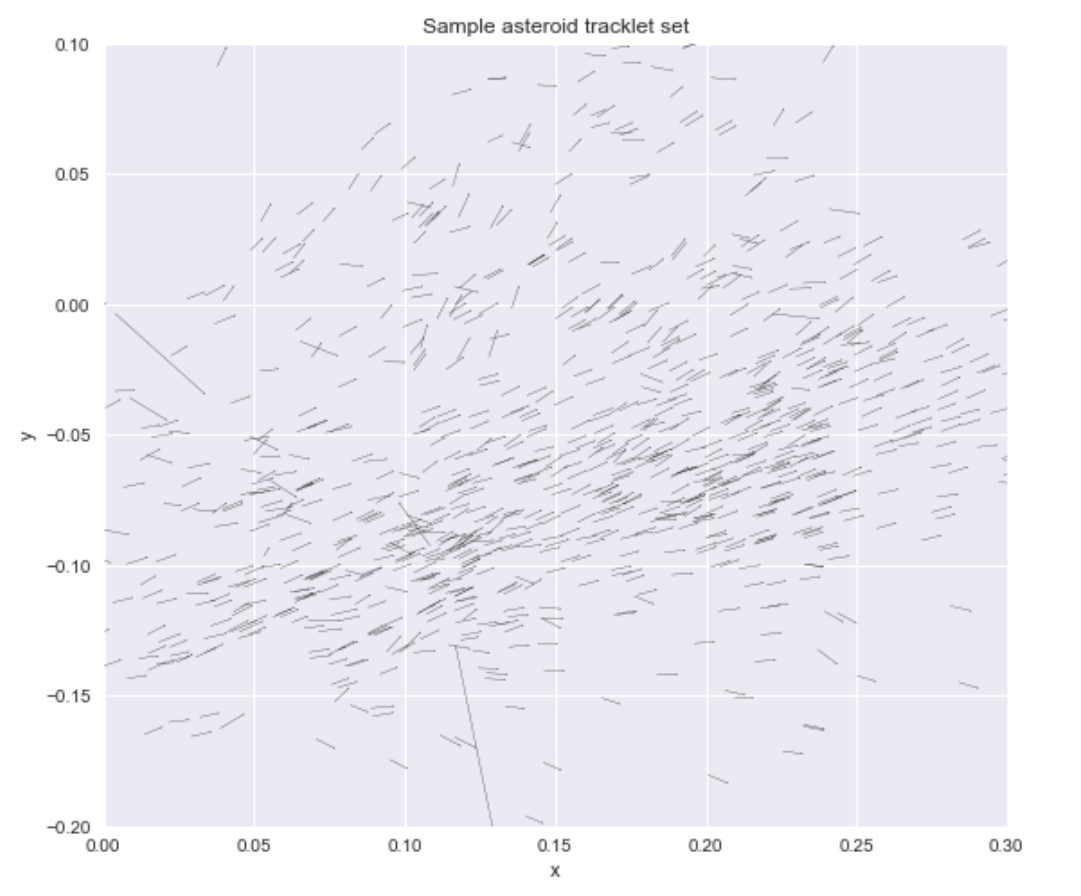
\includegraphics[width=7cm]{3_Final_write_up/1a_unclusters_img.png} }}%
    \qquad
    \subfloat[Identified clusters]{{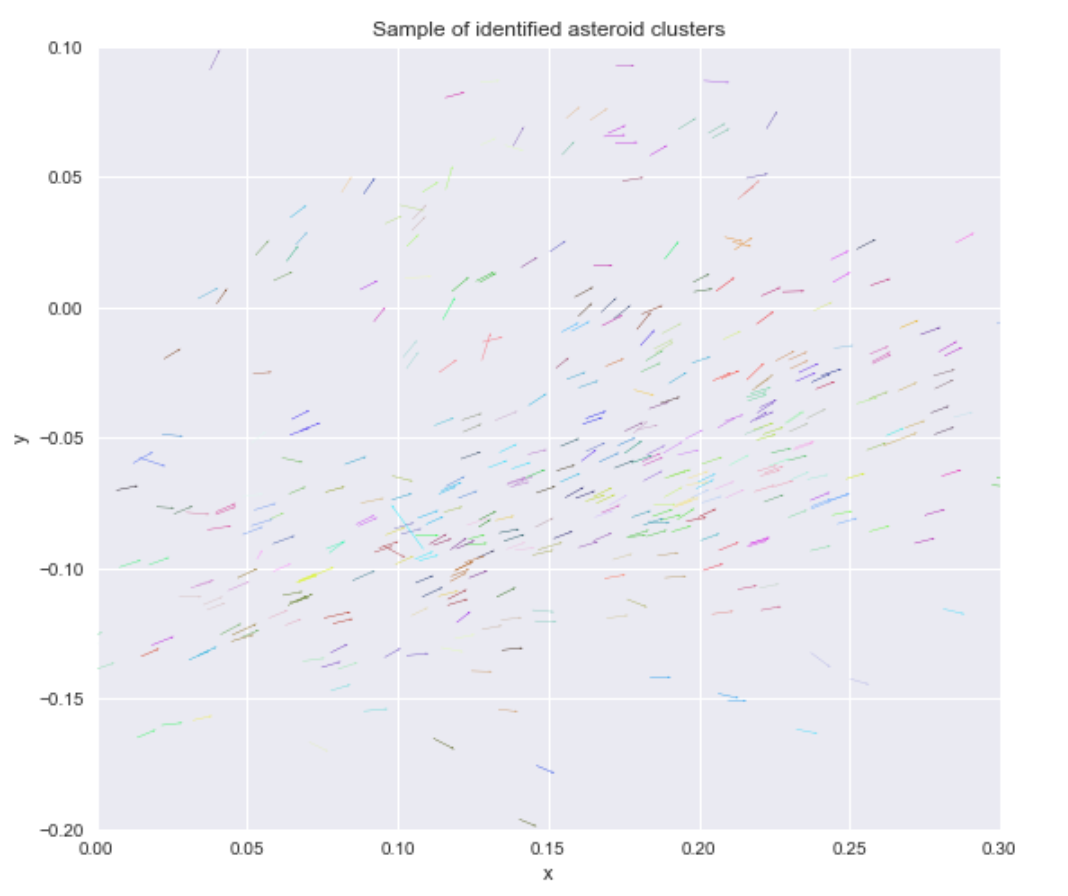
\includegraphics[width=7cm]{3_Final_write_up/1b_clusters_img.png} }}%
    \caption{Asteroid tracklets observed (from the sun) in a small section of space, and identified clusters}%
    \label{fig:clustering}%
    \end{figure}
    \begin{figure}[!hbp]%
    \centering
    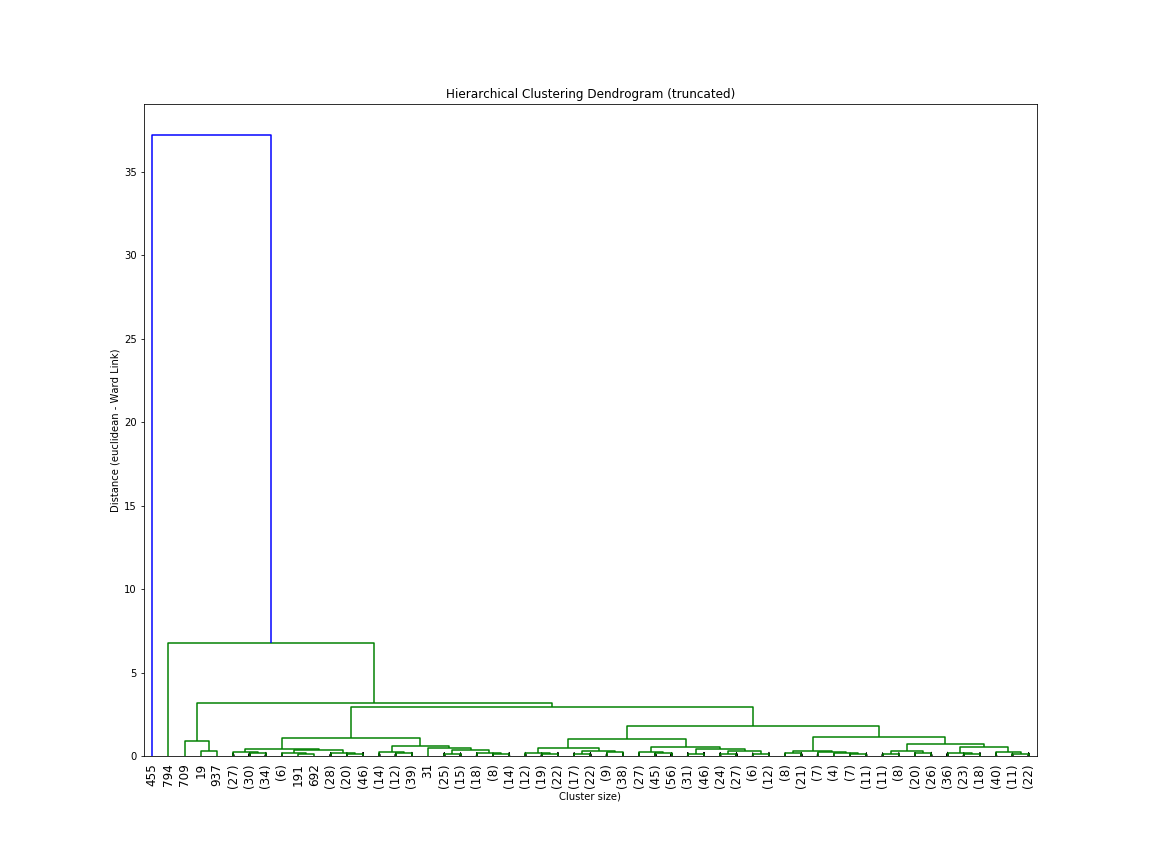
\includegraphics[width=10cm]{3_Final_write_up/3_dendrogram_img.png}
    \caption{Sample cluster topography (distance between groups of clusters - truncated (agglomerative clustering approach)}%
    \label{fig:dendogram}%
    \end{figure}
    \item \textbf{Verify asteroid with orbit fit}\newline
    An orbit fit is computationally expensive to iterate over every possible tracklet combination.  However, it is fortunately sufficiently efficient to perform over the list of expected asteroids produced by the KD-tree clustering.  Therefore, each matched cluster has an orbit fit performed to verify it is indeed matches a possible asteroid trajectory.  
\end{enumerate}

As the clustering functions in $O(n\log(n)$ time, each time/space window can in fact be clustered in approximately five minutes on a standard computer. Although we originally intended to carry out this work on the Odyssey cluster, we found that to be unnecessary.   This is remarkable, given that the conventional solution (MOPS) is deployed on large computing clusters and still struggles.
    
    \subsection{Training Hyperparameters}
We optimize the clustering algorithm by tuning two hyperparameters:
\begin{itemize}
    \item $dt$: Velocity weighting of the cluster.  Given that the clusters are often moving with similar velocities around the sun (but more disparate positions), it is helpful to assign the velocity a higher sensitivity than location when clustering.  
    \item $d$: Clustering radius in four-dimensional space.
\end{itemize}
The velocity weighting was tuned with a physical approach.  We found that the ideal ratio corresponds to the time span of the observations $\pm 15$~days.   This matches positional uncertainty with that from the velocity uncertainty.

The ideal clustering radius was tuned with a labeled training data set of known asteroid trajectories, provided by Matt Payne with the MPC.  \newline
To tune the clustering radius, the training set was divided into five time slices, and the number of correctly identified clusters was counted at each radii, subject to a restriction that there must be $<0.1\%$ spurious tracklet assignments.  That is, the loss function was the number of missed asteroids at a $ 0.1\%$ misclassification rate).

This was repeated at each of the five independent time slices in a 5-fold cross validation to avoid overfitting.  Total runtime was c.100 minutes on a Macbook Pro.  The cluster radius that minimize the loss function was found to be 0.00124 radians, which is the value used in the final ITF clustering.

\section*{Empirical Results}
\subsection*{Accuracy results - Training set}
The training set is fully labelled and asteroid fits are not required for verification of results.\newline
The number of clusters identified versus the number of on the training set is shown in the figure below.  This data is specifically the number of clusters identified over a full iteration of all possible $\dot{z}$ values, in a single time/space "window" of the night sky.

The clustering performed admirably - under the right hyperparameters, the KD-tree successfully identified 80\% of all asteroids on the training data with$ <0.1\%$ spurious clusters identified.

The rationale for the 0.00124 radian clustering value is also evident in the results below - the right-hand graph shows that 0.00124 radian clusters is the ``elbow'' point at which tracklets start to be added spuriously to false clusters.  Our overall estimated estimated classification ROC is also included following:
\begin{figure}[!hbp]%
    \centering
    \subfloat[Number of clusters correctly  identified \newline(blue dashed line = perfect)]{{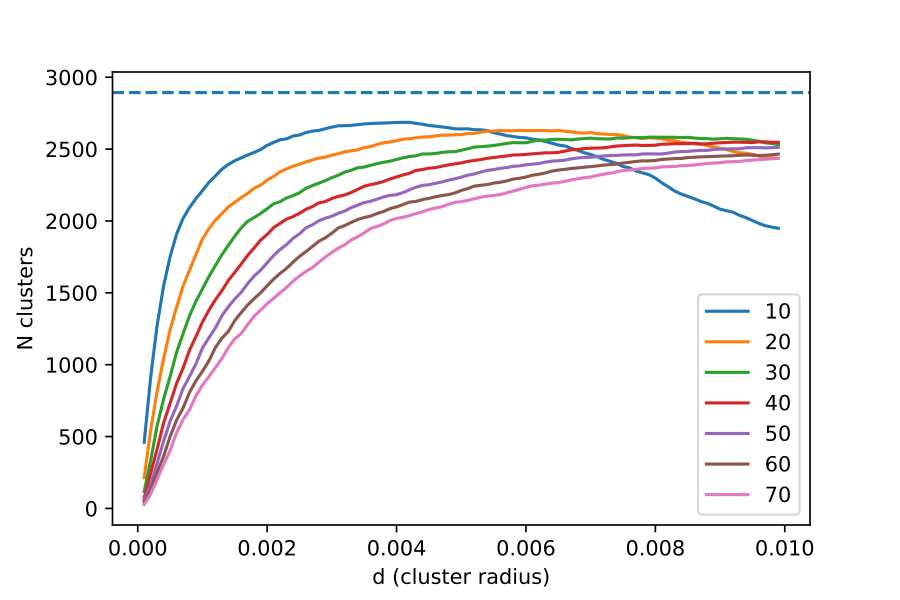
\includegraphics[width=7cm]{3_Final_write_up/4a_nclusters_img.png} }}%
    \qquad
    \subfloat[Number of clusters with at least one erroneous tracklet]{{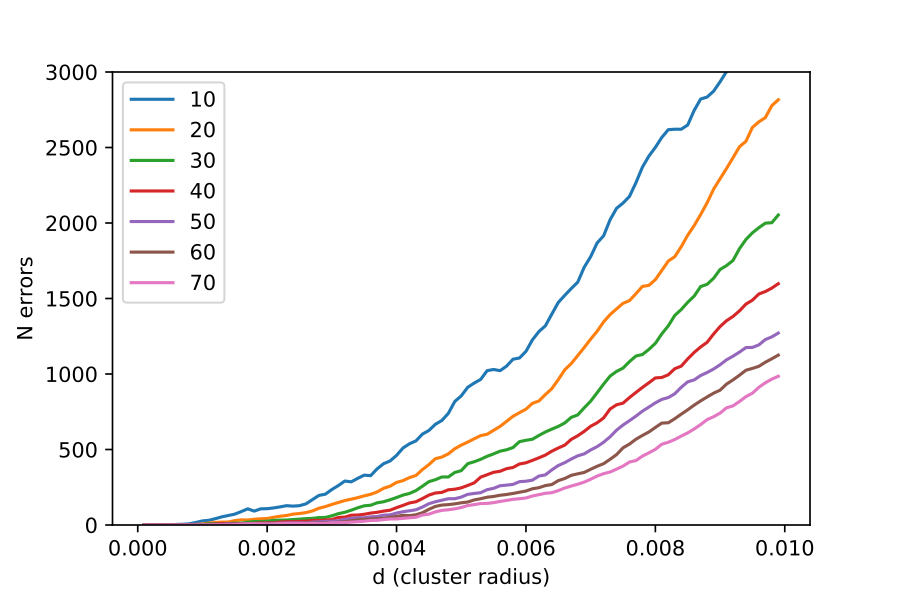
\includegraphics[width=7cm]{3_Final_write_up/4b_nerrors_img.png} }}%
    \caption{Number of correctly identified asteroids versus number of errors (at one region/time of the provided training set)\newline(line colors = $dt$ hyperparameter (in units of days), x-axis = cluster radius hyperparameter, in radians)}%
    \label{fig:accuracy}%
\end{figure}
\begin{figure}[!hbp]%
    \centering
    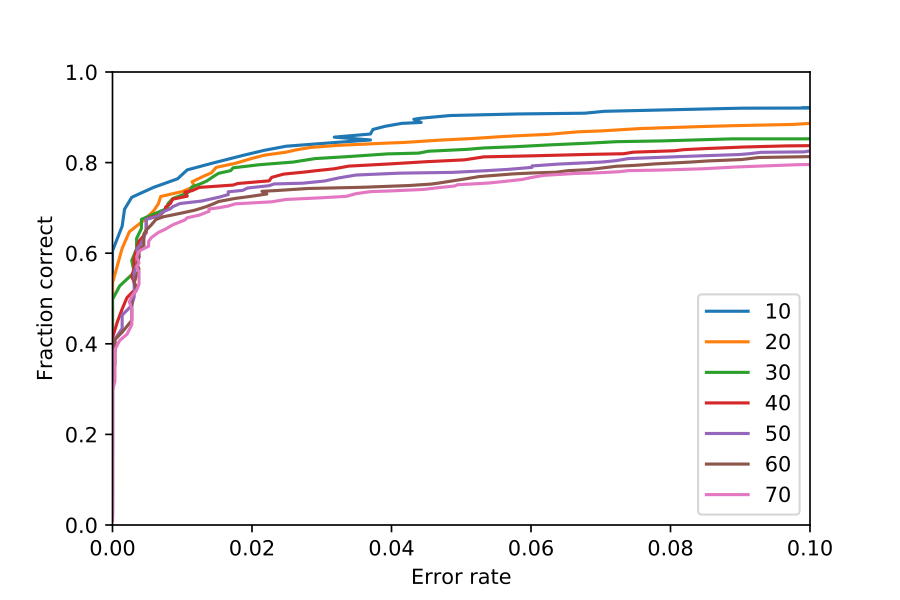
\includegraphics[width=10cm]{3_Final_write_up/5_ROC_asteroids_img.png}
    \caption{ROC Curve for cluster classification.  Note: this is not a binary classification, so the error rate is not the complement of the success rate.}%
    \label{fig:roc}%
\end{figure}
\subsection*{A note on ITF testing accuracy}
The asteroid problem is fortunate in that it has a relatively straightforward method for testing cluster accuracy.  Even in the unlabelled ITF, it is possible to verify an asteroid cluster by performing an orbit fitting calculation.  Orbits are relatively sparse in the night sky so it is unlikely that a spurious asteroid will result in a working orbit.  And while the orbit fitting algorithm is expensive to iterate over all possible asteroid combinations, it can be used to verify the veracity of all asteroids that have been clustered by the KD-tree algorithm overnight on Odyssey.\newline
Therefore, although this is an as-yet-unsolved, unlabeled problem, the accuracy of the solution can be confidently verified.
\subsection*{ITF testing results}
    Although the algorithm performed well on the training set, there was one structural difference between the training dataset and the ITF that was difficult to control for.  Namely, the ITF an order of magnitude higher tracklet density than the training set.  We estimate the ITF tracklet density of c.10-30 tracklets/degree$^2$. 
    
    There was a distinct possibility that the algorithm would fail in either accuracy or computational time as the tracklet density increased (much like previous MOPS attempts had encountered earlier).
    
    Fortunately, the algorithm performed admirably on the higher-density tracklet data!  After removing some duplicated tracklets (as discussed in the conclusions section below), each asteroid detected by the algorithm was able to be correctly orbit-fitted.  Thus far, in a single calculated time window, a total of several hundred asteroids have been discovered with fewer than ten errors. A sample clustering diagram on one slice of the full ITF is below:
    \begin{figure}[!htp]%
    \centering
    \subfloat[Unclustered ITF tracklets.  The tracklets are color coded by time.]{{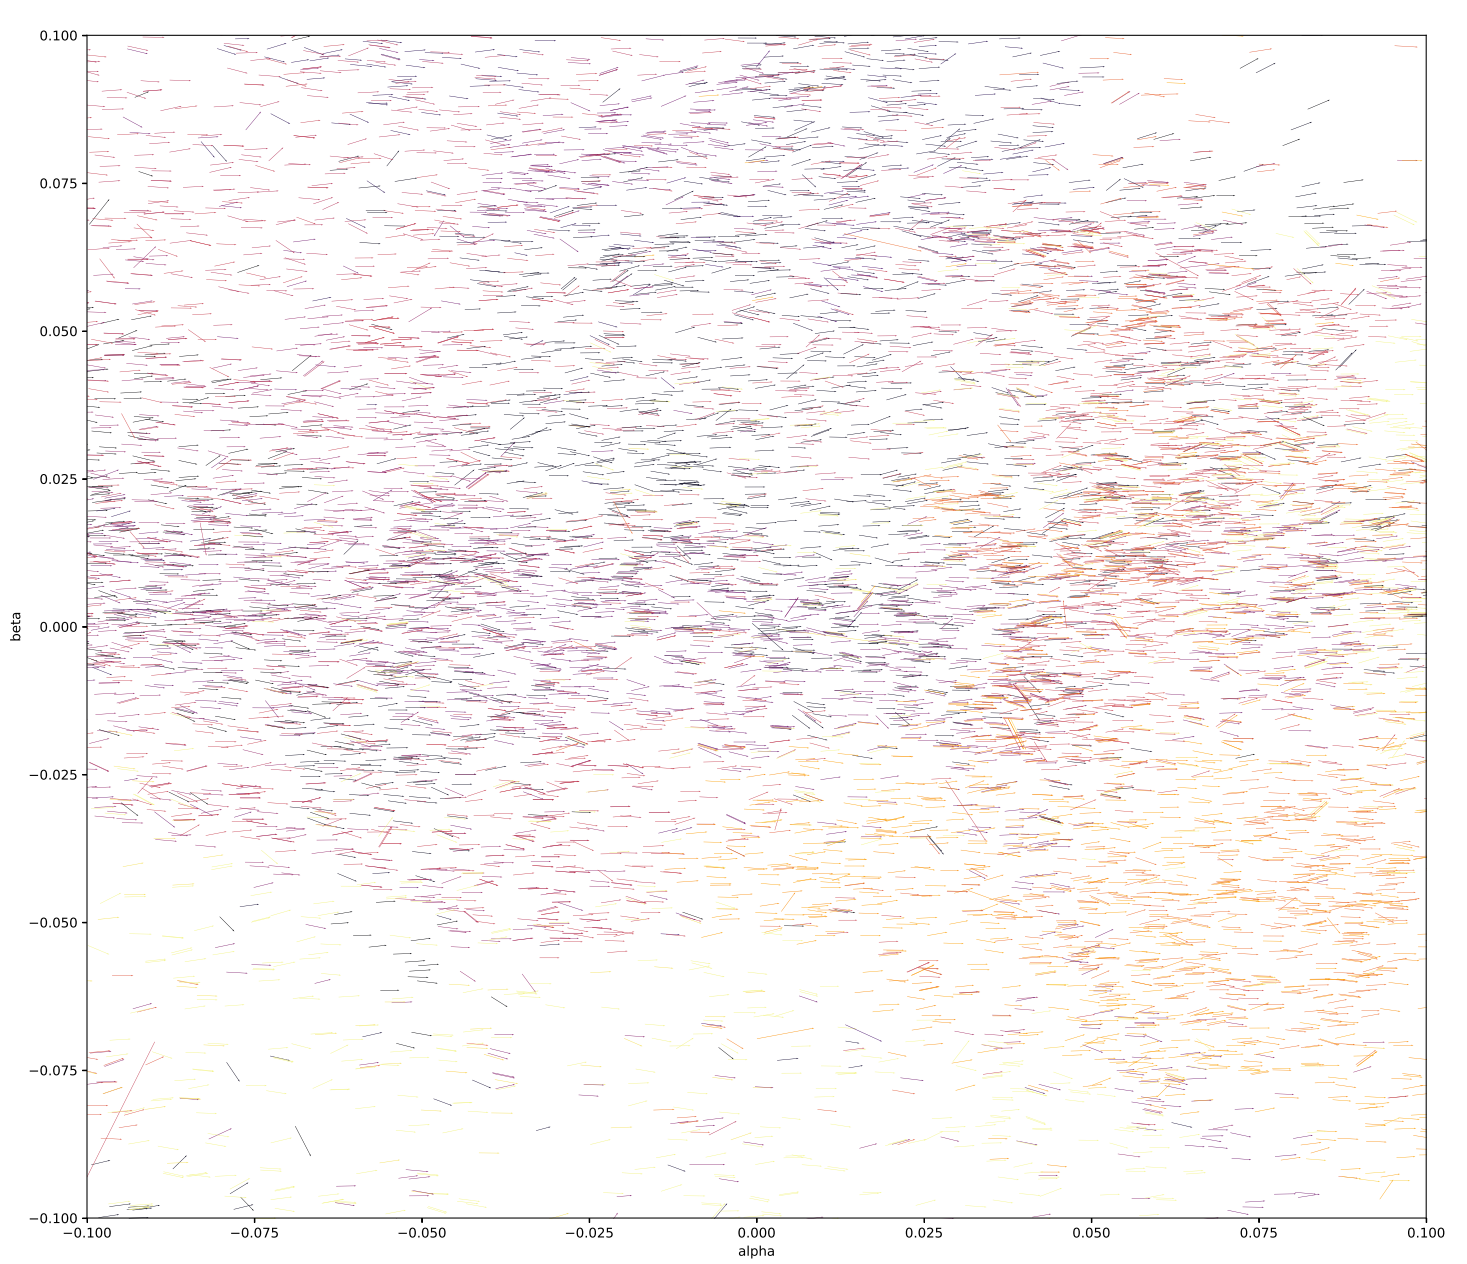
\includegraphics[width=7cm]{3_Final_write_up/7a_itf_asteroids.png} }}%
    \qquad
    \subfloat[Clustered ITF tracklets with KD-tree nearest neighbours.  Each cluster has at least three member tracklets, which are color coded by cluster ID.  The singletons and tracklet pairs, with dominate the left panel,  have been identified and  removed.]{{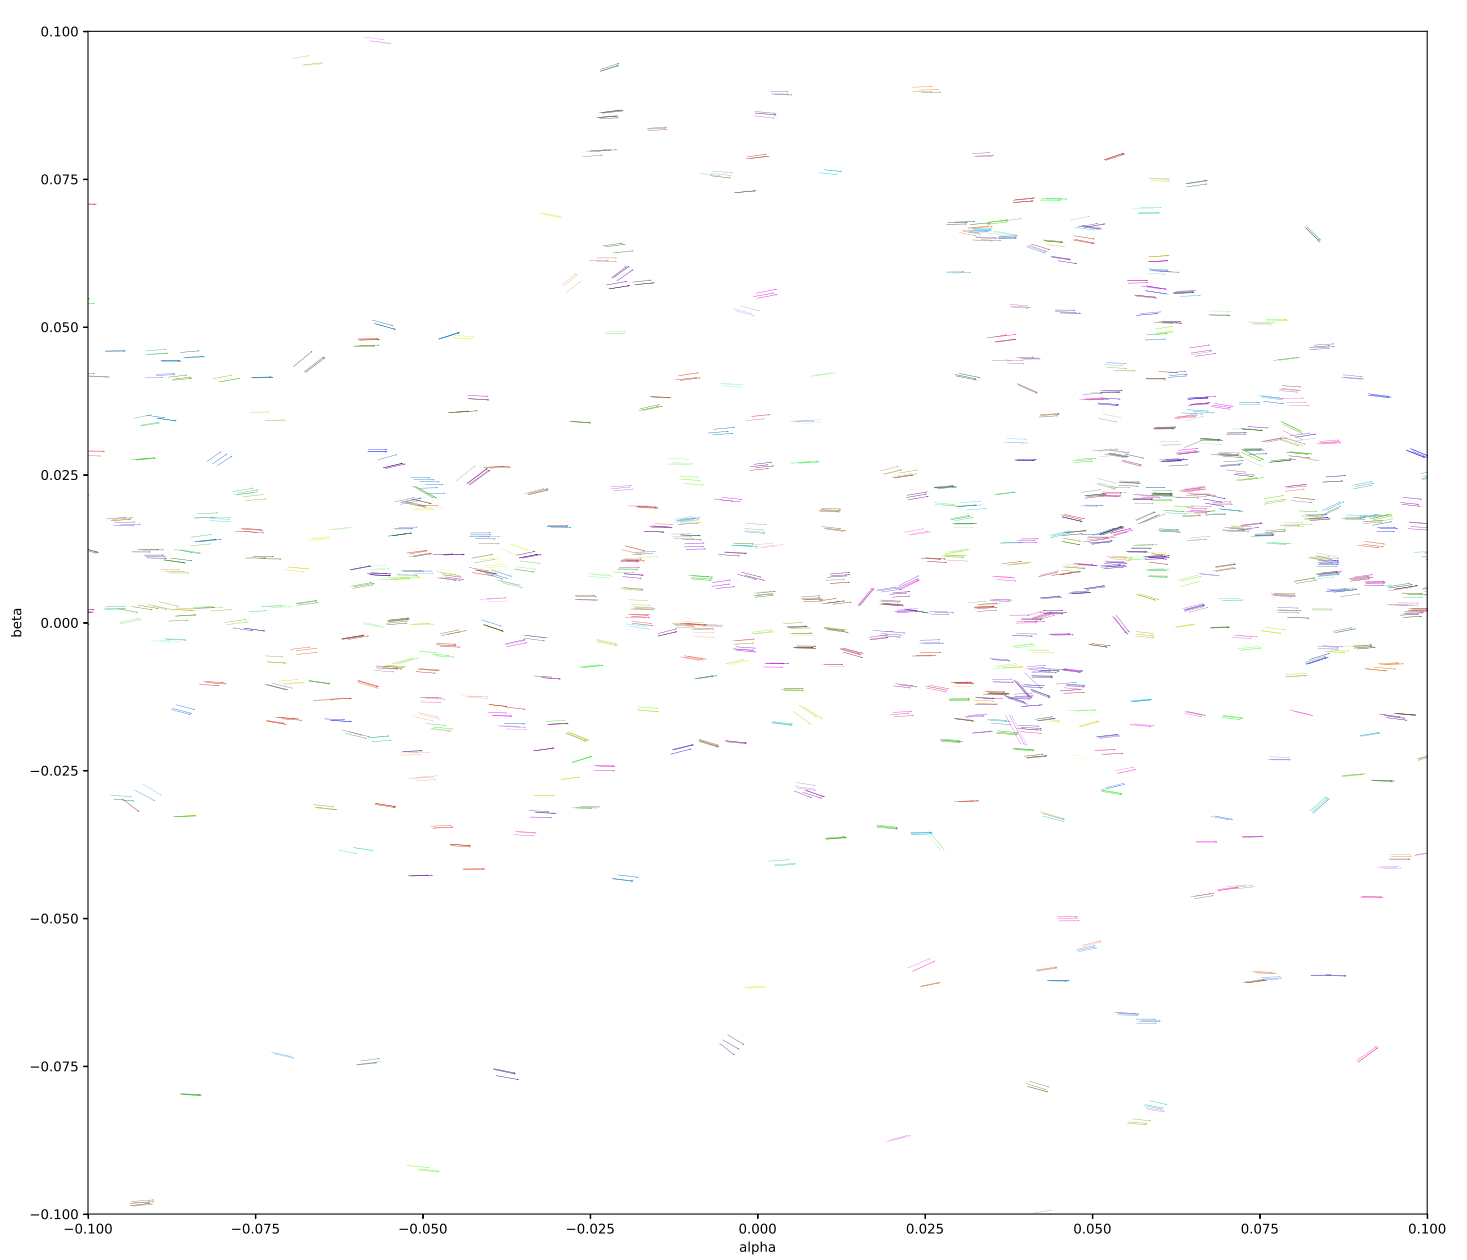
\includegraphics[width=7cm]{3_Final_write_up/7b_itf_clusters.png} }}%
    \caption{Successful ITF clustering}%
    \label{fig:clustering}%
\end{figure}
\newpage
\section*{Conclusions and Next Steps:}
    We have been pleasantly surprised by the efficacy of our algorithm and are very satisfied with the results - in addition to correctly identifying five new asteroids, we have met our ``stretch goal'' of collapsing the ITF and identifying the vast majority of unmatched tracklets in the night sky!

    Our current approach has some limitations that we would address as next steps.  Firstly, observatories can produce tracklet observations at identical times, which our algorithm does not account for.  This does not impair accuracy (these identical observations are clustered as expected), however it causes issues with the legacy orbit-fitting software.  As a next step, we would include a secondary check to filter out identical tracklets to allow for easier orbit-fitting.

    Secondly, our approach works best with a narrow time window.  We currently use $\pm$15 days from the new moon, because secondary effects become more prominent for larger time windows.  For example, for larger time horizons, our assumption of a constant distance becomes invalid because the asteroids follow elliptical orbits.  If we were able to add second-order calculations into our algorithm, larger time windows (and, consequently, reduced computation times) could be possible.

    Finally, our method results in iterating over $\dot{z}$ and clustering in the remaining four dimensions.  This is an intuitive approach, however we believe similar results may be obtained by simply performing a five-dimensional clustering.  This would require us to design additional hyperparameters (specifically, the importance ratio of $\dot{z}$ versus other hyperparameters), but may offer gains in computational speed and accuracy.

    After completing the ITF problem, we intend to apply this method to simulated asteroid data sets for the Large Synoptic Survey Telescope (LSST) and real data sets from the Pan-STARRS-1 telescope.

    Overall, though, we are pleased with the capabilities of the clustering algorithm.  We believe the tool addresses a persistent and growing problem in a computationally tractable manner, with high accuracy and reliability.  

\section*{Acknowledgments}

We thank Scott Kuindersma for originally suggesting that a clustering approach to the asteroid linking problem might be fruitful.  We are grateful to Brian Plancher and the other CS182 teaching staff members for their support and guidance.  

This project is in collaboration with Matt Payne of the MPC.  We thank him for providing a training set and for extensive brainstorming.  We thank Gareth Williams, also of the MPC, for orbit fitting tools.  

We have also benefited from helpful discussions with Timothy Spahr, Jonathan Myers, and David Gerdes.

\section*{References and resources}

\noindent
Panigrahy R (2008), ``An Improved Algorithm Finding Nearest Neighbor Using Kd-trees'', in: Laber E.S., Bornstein C., Nogueira L.T., Faria L. (eds) LATIN 2008: Theoretical Informatics. LATIN 2008. Lecture Notes in Computer Science, vol 4957. Springer, Berlin, Heidelberg\neline\newline

\noindent
Kubica J, Denneau L, Grav T, et al (2007), ``Efficient intra- and inter-night linking of asteroid detections using kd-trees'', Icarus, 189, 151-168.\newline

\noindent
Mashiku A, and Garrison JL (2012), ``Statistical Orbit Determination using the Particle
Filter for incorporating Non-Gaussian Uncertainties'', AIAA Astrodynamics Specialist Conference, August 13–16 2012, Minneapolis, MN, USA.\newline

\noindent
Peter Veres and Steven R. Chesley (2017), ``Near-Earth object linking with the large synoptic survey telescope'', Submitted to AJ, 2017.\newline

\newpage
\section*{Installing and running}

\begin{verbatim}

The repository with our code and installation instructions is located at:

https://github.com/pblankley/itf_linking

Note: This project uses Python 3. 

Install instructions:
$ git clone https://github.com/pblankley/itf_linking.git

Once you have the repo cloned, there are a few libraries you will need to install.
Run the following commands from the command line if you do not have these packages installed.

$ pip install novas
$ pip install novas_de405

Here is the reference for the novas library:

Barron, E. G., Kaplan, G. H., Bangert, J., Bartlett, J. L., Puatua, W., 
Harris, W., & Barrett, P. (2011) 
“Naval Observatory Vector Astrometry Software (NOVAS) Version 3.1, 
Introducing a Python Edition,” Bull. AAS, 43, 2011.

Other than these packages, it is expected that the user has the 
usual python numerical libraries.

Once you have these installed, go to the linkitf directory of 
the repo and run the demo.py file.

\end{verbatim}

\newpage
\section*{Roles and contributions}
Matt Holman: Provided expertise in astronomy, heliocentric math, prepared final iterative methodology, read the paper which was the genesis of this concept 17 years ago, and general superstar


\noindent
Paul Blankley: Supported clustering algorithms, designed demo code, produced amazing visualizations, and kept the ring in sight

\noindent
Ryan Janssen: Supported clustering algorithms, designed hyperparameter tuning strategy, ruled the presentation

\noindent
All: Preparation of reports and presentation
\end{document}